上記の課題を踏まえ、高齢者が生活用品を手軽に確保でき、かつ学生の働き口を増やせる画期的な手段として、我々StellarWorksはインターネットに接続可能な端末から気軽に利用できる Stellar Delivery を提案する。
本アプリは、欲しいものを依頼すると、その商品をお店側と連携して学生が配達してくれるというものである。

\subsection{解決されると考えられる事象- 移動手段の確保問題}

小節1.2および1.3で述べたように、現在、多くの人々が生活用品を確保する際に「移動手段がない」「移動販売が少ない」といった課題に直面しており、このような状況は、少子高齢化の進行や地域交通網の縮小に伴い、今後さらに深刻化することが予想される。

そこで、我々が考案したシステムを活用することで、利用者は自宅にいながら簡単な操作で必要なものを注文し、配達を受けることが可能となる。
これにより、移動の負担を大幅に軽減し、買い物困難者の生活の質向上に寄与できると考えられる。

さらに本システムは、高齢者だけでなく、体調不良や病気、事故、子育てなどの理由で外出が難しい人々にとっても有効な支援手段となりうると考えられる。 

また、高知工科大学の学生102名にアンケート調査を行い、「我々が提案するデリバリーサービスを依頼側として使用したいか」という質問をしたところ、全体の77.4\%から肯定的な意見が得られた。(図 \ref{fig:アンケート2}) 
このため学生からの需要も十分にあると考えられる。 

\begin{figure}[H]
  \centering
  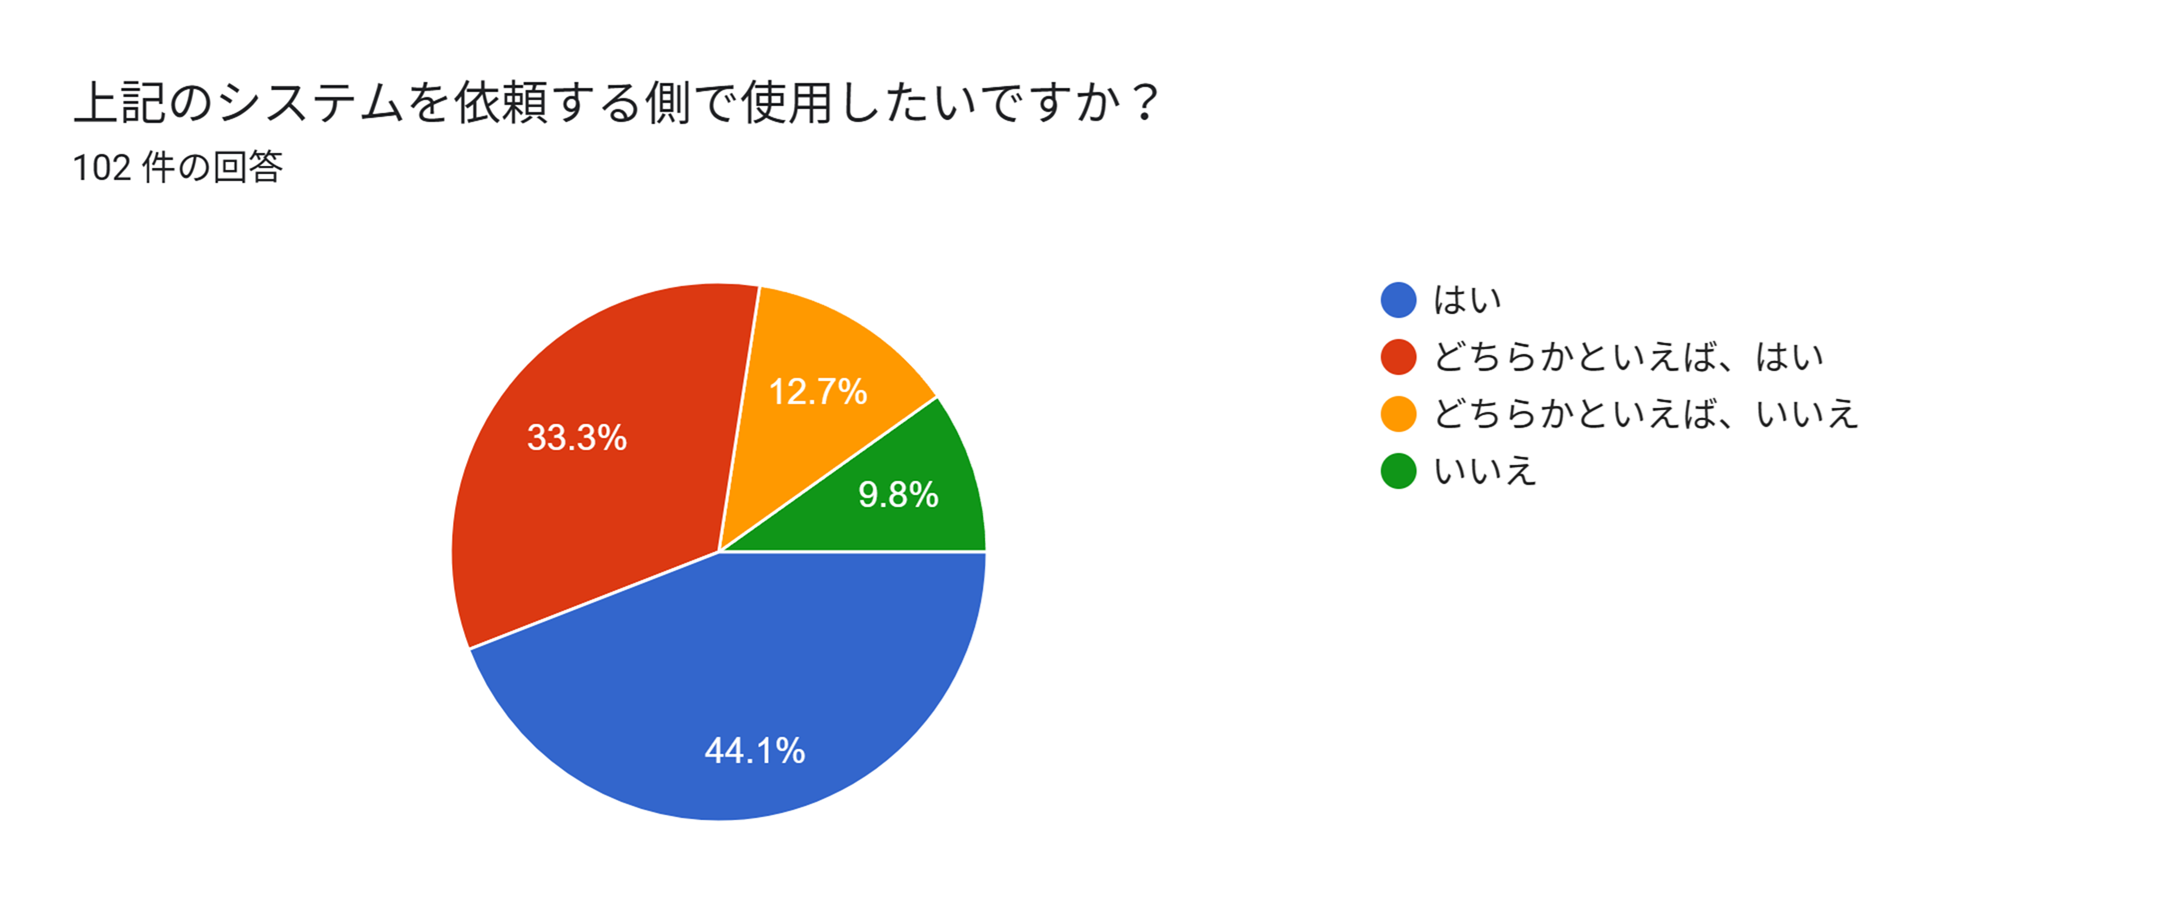
\includegraphics[width=0.75\textwidth]{依頼する側として使用したいか_アンケート結果.png}
  \caption{依頼する側として使用したいかのアンケート調査結果}
  \label{fig:アンケート2}
\end{figure}

%生活用品の確保問題がコメントアウトされている理由
%移動手段の確保問題と内容が被る可能性があるため、それぞれで分けるよりも1つにまとめる方が良いかも

%\subsection{解決されると考えられる事象- 生活用品の確保問題}



\subsection{解決されると考えられる事象- 香美市のアルバイト先の枯渇問題}
%アンケート結果より記述された小節1.3を参考
小節1.4で述べたように、現在の香美市では、学生が働けるアルバイト先が少なく、仕事を見つけづらい状況が続いている。
これは地域の店舗数の減少や人員の削減などが原因で、学生にとっても地域にとっても大きな課題となっている。
そこで、我々が提案するシステムを活用することで、この問題を解消できる可能性があると考えられる。
このサービスでは、商品の配達を学生が担当できるため、新しいアルバイトの場を作り出すことができる。
また、学生にとっては空いた時間を使って働ける柔軟な働き方が可能となり、地域にとっても若者の活躍の場が増えることで活性化につながる。
こうした仕組みにより、香美市のアルバイト不足の問題を解決し、地域全体を元気にすることが期待される。



